\documentclass{beamer}
\usepackage{amsmath,amsbsy,amsopn,amstext,amsfonts,amssymb}
\usepackage{isomath}
\usepackage{ulem}
%\linespread{1.6}  % double spaces lines
\usepackage{graphicx}
\usepackage{subfigure}
\usepackage{color}
\usepackage{optidef}  % define optimization problems
\usepackage{multicol}  % multiple columns
\usepackage{listings} % for python code
\usepackage{mathrsfs}

\usepackage{polynom}
\newcommand{\adj}{\mathrm{adj}}
\newcommand{\constrainedmin}[3]{
		\begin{mini*}|s|
		{#2}{#1}{}{}
		\addConstraint{#3}
		\end{mini*}
}

\newcommand{\rwbcomment}[1]{{\color{blue}RWB:#1}}
\newcommand{\defeq}{\stackrel{\triangle}{=}}
\newcommand{\abs}[1]{\left|#1\right|}
\newcommand{\norm}[1]{\left\|#1\right\|}
\newcommand{\iprod}[1]{\left<#1\right>}
\newcommand{\ellbf}{\boldsymbol{\ell}}
\newcommand{\nubf}{\boldsymbol{\nu}}
\newcommand{\mubf}{\boldsymbol{\mu}}
\newcommand{\abf}{\mathbf{a}}
\newcommand{\bbf}{\mathbf{b}}
\newcommand{\cbf}{\mathbf{c}}
\newcommand{\dbf}{\mathbf{d}}
\newcommand{\ebf}{\mathbf{e}}
\newcommand{\fbf}{\mathbf{f}}
\newcommand{\gbf}{\mathbf{g}}
\newcommand{\hbf}{\mathbf{h}}
\newcommand{\ibf}{\mathbf{i}}
\newcommand{\jbf}{\mathbf{j}}
\newcommand{\kbf}{\mathbf{k}}
\newcommand{\lbf}{\mathbf{l}}
\newcommand{\mbf}{\mathbf{m}}
\newcommand{\nbf}{\mathbf{n}}
\newcommand{\obf}{\mathbf{o}}
\newcommand{\pbf}{\mathbf{p}}
\newcommand{\qbf}{\mathbf{q}}
\newcommand{\rbf}{\mathbf{r}}
\newcommand{\sbf}{\mathbf{s}}
\newcommand{\tbf}{\mathbf{t}}
\newcommand{\ubf}{\mathbf{u}}
\newcommand{\vbf}{\mathbf{v}}
\newcommand{\wbf}{\mathbf{w}}
\newcommand{\xbf}{\mathbf{x}}
\newcommand{\ybf}{\mathbf{y}}
\newcommand{\zbf}{\mathbf{z}}
\newcommand{\Jbf}{\mathbf{J}}
\newcommand{\Acal}{\mathcal{A}}
\newcommand{\Bcal}{\mathcal{B}}
\newcommand{\Lcal}{\mathcal{L}}
\newcommand{\Ncal}{\mathcal{N}}
\newcommand{\Rcal}{\mathcal{R}}
\definecolor{darkolivegreen}{rgb}{0.33, 0.42, 0.18}

\makeatletter
\newenvironment<>{proofstart}[1][\proofname]{%
    \par
    \def\insertproofname{#1\@addpunct{.}}%
    \usebeamertemplate{proof begin}#2}
  {\usebeamertemplate{proof end}}
\newenvironment<>{proofcont}{%
  \setbeamertemplate{proof begin}{\begin{block}{}}
    \par
    \usebeamertemplate{proof begin}}
  {\usebeamertemplate{proof end}}
\newenvironment<>{proofend}{%
    \par
    \pushQED{\qed}
    \setbeamertemplate{proof begin}{\begin{block}{}}
    \usebeamertemplate{proof begin}}
  {\popQED\usebeamertemplate{proof end}}
\makeatother

\title{ECEn 671: Mathematics of Signals and Systems}
\author{Randal W. Beard}
\institute{Brigham Young University}
\date{\today}

\begin{document}

%-------------------------------
\begin{frame}
	\titlepage
\end{frame}

%%%%%%%%%%%%%%%%%%%%%%%%%%%%%%%%%%%%%%%%%%%%%%%%%%%%%%%%%%%%%%%%%
\section{Gradient Descent}
\frame{\sectionpage}


%----------------------------------
\begin{frame}\frametitle{Gradient Descent}
	The topic for the remainder of the course is minimization and maximization of functions.
	
	\vfill
	
	In particular we will constrain our attention to continuously differentiable functions.
\end{frame}

%----------------------------------
\begin{frame}\frametitle{Gradient Descent}
	Suppose we have a function of the form
	\begin{center}
		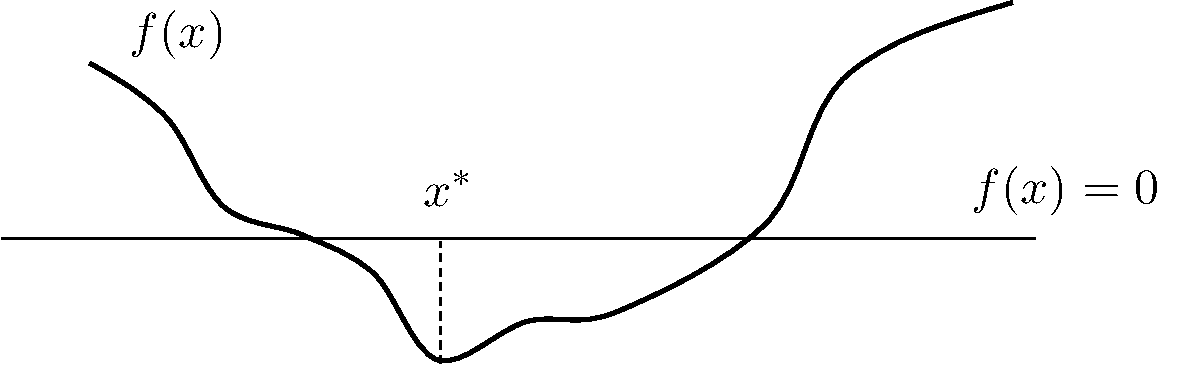
\includegraphics[width=0.5\textwidth]
			{figures/chap14_function_with_minimum}
	\end{center}
	and we would like to find $x^{\ast}$, what should we do?
\end{frame}

%----------------------------------
\begin{frame}\frametitle{Gradient Descent}
	The basic idea of gradient descent is to pick any $x^{[0]}$ and then move ``downward''.  To move down, we look at the slope of $f$.
	
	\vfill
	
	If $\frac{\partial f}{\partial x}(x^{[k]})$ is positive, chose $x^{[k+1]} < x^{[k]}$.
	
	\vfill
	
	If $\frac{\partial f}{\partial x}(x^{[k]})$ is negative, choose $x^{[k+1]} > x^{[k]}$
	
	\vfill
	
	i.e.
	\[ 
		x^{[k+1]} = x^{[k]} - \alpha \frac{\partial f}{\partial x}(x^{[k]}),
	\]
	where $\alpha$ is the step size.	
\end{frame}

%----------------------------------
\begin{frame}\frametitle{Gradient Descent}
	Before moving to the multivariable case, lets consider the potential problems with this approach.	
	
	\vfill
	
	{\color{blue}Problem 1: Local Minima.}
	If $f$ looks like this:
	\begin{center}
		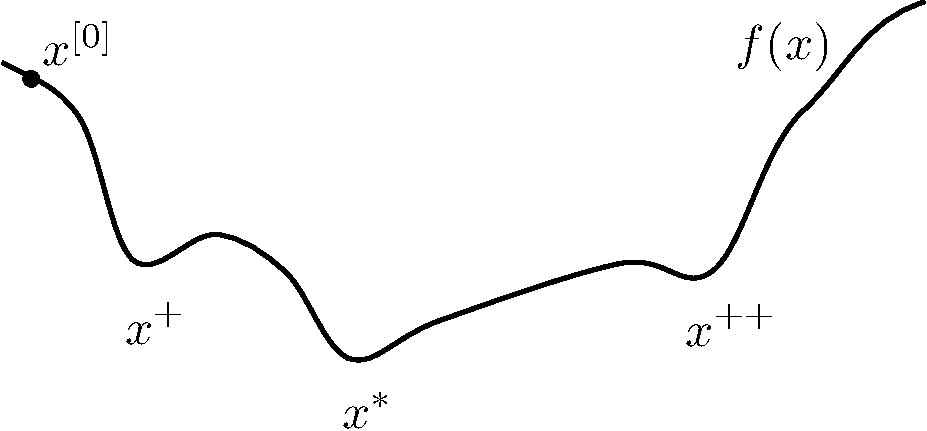
\includegraphics[width=0.5\textwidth]
			{figures/chap14_function_gradiant_descent}
	\end{center}
	then if the initial condition is at $x^{[0]}$, the iteration 
	\[
		x^{[k+1]} = x^{[k]} - \alpha \frac{\partial f}{\partial x}(x^{[k]})
	\] 
	will converge to $x^+$, if $\alpha$ is small enough.
\end{frame}

%----------------------------------
\begin{frame}\frametitle{Gradient Descent}
	Other initial conditions will result in 
	$x^{++}$ while others will give $x^\ast$, the true minimum.
	
	\vfill
	
	This is a fundamental problem with \underline{any} method that relies on derivative information.  There are no completely satisfactory solutions to the problem.  However there are many ad-hoc fixes.	

	\vfill
	
	\begin{example}
		\begin{itemize}
		\item Execute from numerous ``random'' initial conditions and pick the lowest solution.
		\item Occassionally introduce random jumps in $x$.
		\item etc...
		\end{itemize}
	\end{example}
\end{frame}

%----------------------------------
\begin{frame}\frametitle{Gradient Descent}
	{\color{blue}Problem 2: Step Size.}
	The selection of $\alpha$ can have a major effect on the convergence of the sequence
	\[ 
		x^{[k+1]} = x^{[k]} - \alpha \frac{\partial f}{\partial x}(x^{[k]}) 
	\]
	
	For example,
	\begin{center}
		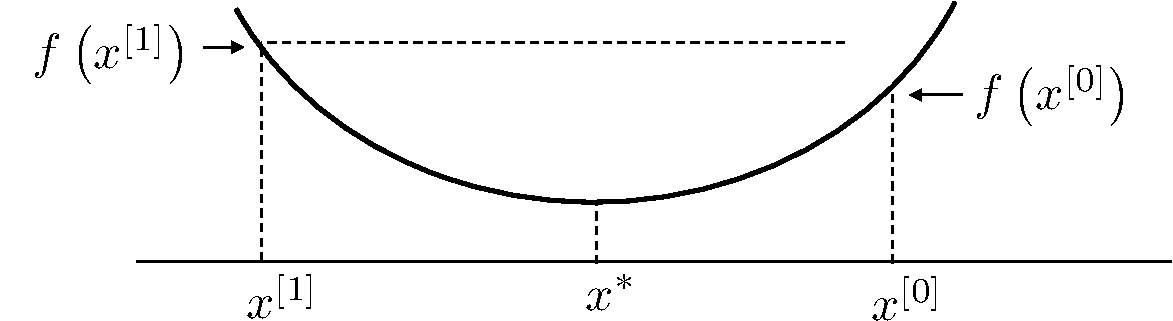
\includegraphics[width=0.5\textwidth]
			{figures/chap14_quadratic}
	\end{center}
	Note $f$ is very steep on sides, so $\alpha \frac{\partial f}{\partial x}(x^{[k]})$ could be large.  This could cause $x^{[1]}$ to overshoot the minimum.  This could cause (1) instability, (2) limit cycles, (3) extremely slow and oscillatory convergence	
\end{frame}

%----------------------------------
\begin{frame}\frametitle{Gradient Descent}

	{\color{blue}Lesson:}  
		Don't make $\alpha$ too large.
		
	\vfill
	
	However if $\alpha$ is too small, then convergence will be very slow.
	
	\vfill
	
	Most implementations adapt the size of $\alpha$.
\end{frame}

%%%%%%%%%%%%%%%%%%%%%%%%%%%%%%%%%%%%%%%%%%%%%%%%%%%%%%%%%%%%%%%%%
\section{Gradient Descent: Multivariable Case}
\frame{\sectionpage}

%----------------------------------
\begin{frame}\frametitle{Gradient Descent: Multivariable Case}
	Let $f:\mathbb{R}^n\to\mathbb{R}$ be a multivariable function.
	\begin{example}
		If $x \in \mathbb{R}^n$ then 
		$f(x) = x_1^2 + x_2^2 + \cdots + x_n^2$ maps $\mathbb{R}^n\to\mathbb{R}$.	
	\end{example}
	The gradient of a multivariable function is
	\[ 
		\frac{\partial  f}{\partial  x} = \begin{pmatrix}
	    \frac{\partial  f}{\partial  x_1}\\
	    \vdots\\
	    \frac{\partial  f}{\partial  x_n}
	  \end{pmatrix} 
	\] 
	and maps $\mathbb{R}^n \to \mathbb{R}^n$.
\end{frame}

%----------------------------------
\begin{frame}\frametitle{Gradient Descent: Multivariable Case}
	\begin{example}
		If $f(x) = x_1^2 + \cdots + x_n^2$ then
		\( 
			\frac{\partial  f}{\partial  x} 
				= \begin{pmatrix}
		    		2x_1\\
		    		2x_2\\
		    		\vdots\\
		    		2x_n
		  		  \end{pmatrix}
		\)		
	\end{example}

	\begin{center}
		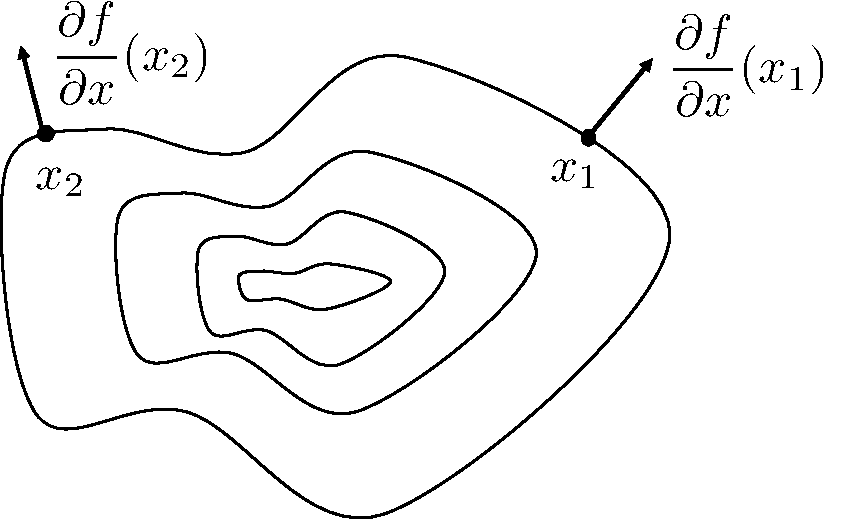
\includegraphics[width=0.5\textwidth]
			{figures/chap14_2D_gradiant}
	\end{center}
	The gradient points perpendicular to the level curves of $f$.	
\end{frame}

%----------------------------------
\begin{frame}\frametitle{Gradient Descent: Multivariable Case}
	\begin{theorem}[Moon Theorem 14.5]
		Let $f:\mathbb{R}^m \to \mathbb{R}$ be a differentiable function in some open set $D$.  The gradient $\frac{\partial  f}{\partial  x}(x)$ points in the direction of the maximum increase of $f$ at the point $x$.		
	\end{theorem}
\end{frame}

%----------------------------------
\begin{frame}\frametitle{Gradient Descent: Multivariable Case}
	\begin{proof}
		Expand $f(x+\lambda y)$ in a Taylor series as
		\[ 
			f(x + \lambda y) = f(x) + \lambda\frac{\partial  f^T}{\partial  x}(x)y + \text{Higher Order Terms (HOT)} 
		\]
		where HOT. are $O(\lambda^2)$, i.e.,
		\[
			\lim_{\lambda \to 0}\frac{H.O.T.}{\lambda} = 0.
		\]	
		We would like to find $y$ that maximizes $f(x + \lambda y)$ as $\lambda \to 0$.

		By Cauchy-Schwartz, $\frac{\partial  f^T}{\partial  x}y$ is maximized when $y = \frac{\partial  f}{\partial  x}$.	
	\end{proof}
\end{frame}

%----------------------------------
\begin{frame}\frametitle{Gradient Descent: Multivariable Case}
	For multivarible functions, the gradient descent formula is
	\[ 
		\fbox{$x^{[k+1]} = x^{[k]} - \alpha_k \frac{\partial f}{\partial x}(x^{[k]})$}
	\]
	
	Again, the selection of the step size is very important.  If $\alpha_k$ is too small convergence will be slow.
	
	\vfill
	
	If $\alpha_k$ is too large, algorithm could be unstable.	
	
	\vfill
	
	How to pick the right $\alpha$?
	
\end{frame}

%----------------------------------
\begin{frame}\frametitle{Gradient Descent: Multivariable Case}
	Locally around a min or max, every smooth function can be approximated by a quadratic (Taylor series).  
	
	\vfill
	
	We can gain insight about the selection of $\alpha$ by studying quadratic functions.
	
	\vfill
	
	Let $f(x) = x^TRx - 2b^Tx$ where $x \in \mathbb{R}^m,b\in\mathbb{R}^m,R=R^T>0$.	
	
	\vfill
	
	Taking the gradient we get
	\[ 
		\frac{\partial f}{\partial x} = 2Rx - 2b.
	\]
\end{frame}

%----------------------------------
\begin{frame}\frametitle{Gradient Descent: Multivariable Case}
	So the gradient descent algorithm is
	\[ 
		x^{[k+1]} = x^{[k]} - 2\alpha(Rx^{[k]} - b). 
	\]
	Let $x^{\ast}$ satisfy $Rx^{\ast}=b$ then
	\[ 
		x^{[k+1]} - x^{\ast} = x^{[k]} - x^{\ast} - 2\alpha(Rx^{[k]} - Rx^{\ast}) 
	\]
	Define $y^{[k]} = x^{[k]} - x^{\ast}$ and $\mu = 2\alpha$, then 
	\begin{align*}
		y^{[k+1]} 
			&= y^{[k]} - \mu R y^{[k]} \\
			&= (I - \mu R)y^{[k]}\\
		\implies y^{[k]} &= (I - \mu R)^ky^{[0]}.
	\end{align*}	
\end{frame}

%----------------------------------
\begin{frame}\frametitle{Gradient Descent: Multivariable Case}
	Since $R$ is symmetric positive definite
	\[ 
		R = Q\Lambda Q^T 
	\]
	where $Q$-orthogonal.
	Therefore,
	\begin{align*}
		y^{[k]} 
			&= (QQ^T-\mu Q\Lambda Q^T)^ky^{[0]}\\
			&= Q(I-\mu\Lambda)^kQ^Ty^{[0]}
	\end{align*}
	Letting $z = Q^Ty$,
	\begin{align}
		& z^{[k]} = (I - \mu\Lambda)^kz^{[0]}\\
		\implies &
		z^{[k]}_i = (1 - \mu \lambda_i)^kz_i^{[0]}
	\end{align}
	which converges if $\abs{1-\mu\lambda_i} < 1$, $i = 1, \ldots, m$.	
\end{frame}

%----------------------------------
\begin{frame}\frametitle{Gradient Descent: Multivariable Case}
	Therefore, convergence happens when
	\begin{align*}
	-1 &< 1 - \mu \lambda_i < 1 \\
	\iff -2 &< -\mu\lambda_i < 0\\
	\iff 0 &< \mu\lambda_i < 2\\
	\iff 0 &< \mu < \frac{2}{\lambda_i} 
	\end{align*}
	Recall that $\lambda_i > 0$ when $R$ is positive definite, 
	so if
	\[ 
		0 < \alpha < \frac{1}{\lambda_{\max}(R)} 
	\]
	then steepest descent converges for quadratic functions.
\end{frame}

%----------------------------------
\begin{frame}\frametitle{Gradient Descent: Multivariable Case}
	Note that the convergence along each eigenaxis is determined by 
	\(
		\frac{1}{\lambda_i}.
	\)	
	
	\vfill

	Therefore if $R$ is ill-conditioned, i.e., $\displaystyle \frac{\lambda_{\max}}{\lambda_{\min}}$ is large, then convergence for gradient descent will be much slower along some axes than others.	
\end{frame}



\end{document}